\documentclass[11pt,addpoints]{exam}
% Lab revised by:
% Aakash N. Maskeri and Nathan Mehaffy
% Assignment Info
\newcommand{\courseno}{18-100}
\newcommand{\coursename}{Intro to Electrical and Computer Engineering}
\newcommand{\fullcoursename}{\courseno: \coursename}
\newcommand{\semester}{Spring 2026}
\newcommand{\assignmenttype}{LAB}
\newcommand{\assignmentnumber}{05}
\newcommand{\assignmentname}{Op-Amp Neural Network}
\newcommand{\assignment}{\assignmenttype \assignmentnumber: \assignmentname}
\newcommand{\due}{TBD}
\newcommand{\demosdue}{TBD}
\newcommand{\cmu}{\copyright{ }Carnegie Mellon University}

% Template package and define image path
\usepackage{ecetemplate}
\graphicspath{{images/}}

\begin{document}
    \begin{coverpages}
    \begin{center}
	\LARGE\textbf{\fullcoursename} 
	\huge{\textbf{\assignment}} \\
	\LARGE{\textbf{Writeup Due: }\due} \\
    \LARGE{\textbf{Checkoffs Due: }\demosdue} \\
	\end{center}
	\begin{tabular}{ll}
		Name: &\rule{0.83\textwidth}{0.4pt} \bigskip \\ 
		Andrew ID: &\rule{0.83\linewidth}{0.4pt} \\
	\end{tabular}

	\medbreak
	\textbf{\large How to submit labs:} 
	
	Download from this file from \emph{Canvas} and edit it with whatever PDF editor you're most comfortable with. Some recommendations from other students and courses that use Gradescope include:
	\vspace{-1\baselineskip}
	\begin{description}[leftmargin=12em,style=nextline,itemsep=0em]

        \item[\href{https://dochub.com/}{DocHub}] An online PDF annotator that works on desktop and mobile platforms.
 
        \item[\href{https://www.pdfescape.com/}{pdfescape.com}] A web-based PDF editor that works on most, if not all, devices. 
		\item[\href{https://www.iannotate.com/}{iAnnotate}] A cross-platform editor for mobile devices (iOS/Android). 
	\end{description}
	\vspace{-1\baselineskip}
	
	\textit{If you have difficulties inserting your image into the PDF, simply append them as an extra page to the END of your lab packet and mark the given box. \textbf{Do NOT insert between pages.}}
	
	If you'd prefer not to edit a PDF, you can print the document, write your answers in neatly and scan it as a PDF. \emph{(Note: We do not recommend this as unreadable lab reports will not be graded!)}. Once you've completed the lab, upload and submit it to \textit{Gradescope}. 
	
	Note that while you may work with other students on completing the lab, this writeup is to be completed alone. Do not exchange or copy measurements, plots, code, calculations, or answer in the lab writeup.
	
	\textbf{\large Your lab grade will consist of two components:}
	\vspace{-\baselineskip}
	\begin{enumerate}
	    \itemsep0pt
		\item Answers to all lab questions in your lab handout. The questions consist of measurements taken during the lab activities, calculations on those measurements and questions on the lab material.
		\item A demonstration of your working lab circuits and conceptual understanding of the material. This demo will occur during office hours.
	\end{enumerate}
    \vspace{-.25cm}
	\begin{center}
		\partialgradetable{credit}[h][questions]
	\end{center}
	\vfill
\end{coverpages}
\pagebreak % shared
    \section{Lab Outline}
In this lab, you will build an analog neural network from op-amp building blocks. Each section teaches a fundamental op-amp circuit, then you will wire them all together into a working 2-2-1 artificial neural network (ANN) that can learn any binary logic function.
\vspace{-\baselineskip}
\begin{enumerate}
    \itemsep0pt
    \item Introduction --- What Are We Building?
    \item Comparator Light Switch
    \item Buffer (Unity-Gain Amplifier)
    \item Amplifiers (Non-Inverting and Inverting)
    \item Inverting Summing Amplifier
    \item Diode Rectifier
    \item Putting It All Together --- The Analog Neural Network
\end{enumerate}

\subsection*{Small Group Check-off Circuits}
\vspace{-1.1\baselineskip}
\begin{todolist}
    \item ANN Circuit --- demonstrate XOR and NAND
\end{todolist}

\vspace{-1.1\baselineskip}
\subsection*{Equipment Required}
\begin{itemize}
    \itemsep0pt
    \item 1x Breadboard
    \item 2x 9V Battery with Battery Clip
    \item 1x Digital Multimeter
    \item 1x AD3 \{\texttt{Power Supply}, \texttt{Oscilloscope}, \texttt{Signal Generator}\}
    \item 1x Wire Strippers
    \item 1x Diagonal Cutters
\end{itemize}

\vspace{-1.1\baselineskip}
\subsection*{Bill of Materials --- Final ANN Circuit (Section 6)}
\begin{tabularx}{\linewidth}{XX}
    3x TL072 Dual Op-Amp IC & 5x 10\si{\kilo\ohm} Linear Pot (\texttt{B10K}) \\
    12x \resistorcode[0.5]{brown}{black}{orange} 10\si{\kilo\ohm} Resistor & 4x \resistorcode[0.5]{yellow}{violet}{red} 4.7\si{\kilo\ohm} Resistor \\
    2x 1N4148 Signal Diode & 1x Red LED \\
    2x SPDT Toggle Switch & 2x 9V Battery + Clip \\
\end{tabularx}

\medbreak
\textit{Additional components for intermediate sections (1--4):}

\begin{tabularx}{\linewidth}{XX}
    1x LDR (CdS cell) --- Section 1 & 1x 20\si{\kilo\ohm} Pot (\texttt{B20K}) --- Section 3 \\
    $\sim$5x \resistorcode[0.5]{brown}{black}{red} 1\si{\kilo\ohm} Resistor --- Sections 1--3 & \\
\end{tabularx}

\vspace{-\baselineskip}
\subsection*{Pinouts}
\begin{figure}[H]
    \hspace{2.1em}\includegraphics[width=0.2\linewidth]{TL072_Pinout.png}

    \hspace{3.1em}TL072 Op-Amp Pinout
\end{figure}

\pagebreak
 % table of contents
    \section{Introduction --- What Are We Building?}

Imagine you want to build a device that can represent \emph{any} mapping from two binary inputs to a binary output. You could hard-wire a specific logic gate, but then you'd have to rebuild the circuit every time you wanted a different function. What if, instead, you could build a single circuit and simply \emph{adjust some knobs} to change what it computes?

This is exactly what a \textbf{neural network} does. A neural network is a system of adjustable \emph{weights}, \emph{summers}, and \emph{cutoffs} that can be ``trained'' to represent any function. In this lab you will build one entirely from analog op-amp circuits.

\subsection*{The 2-2-1 Network}

Our network has the following structure:

\begin{center}
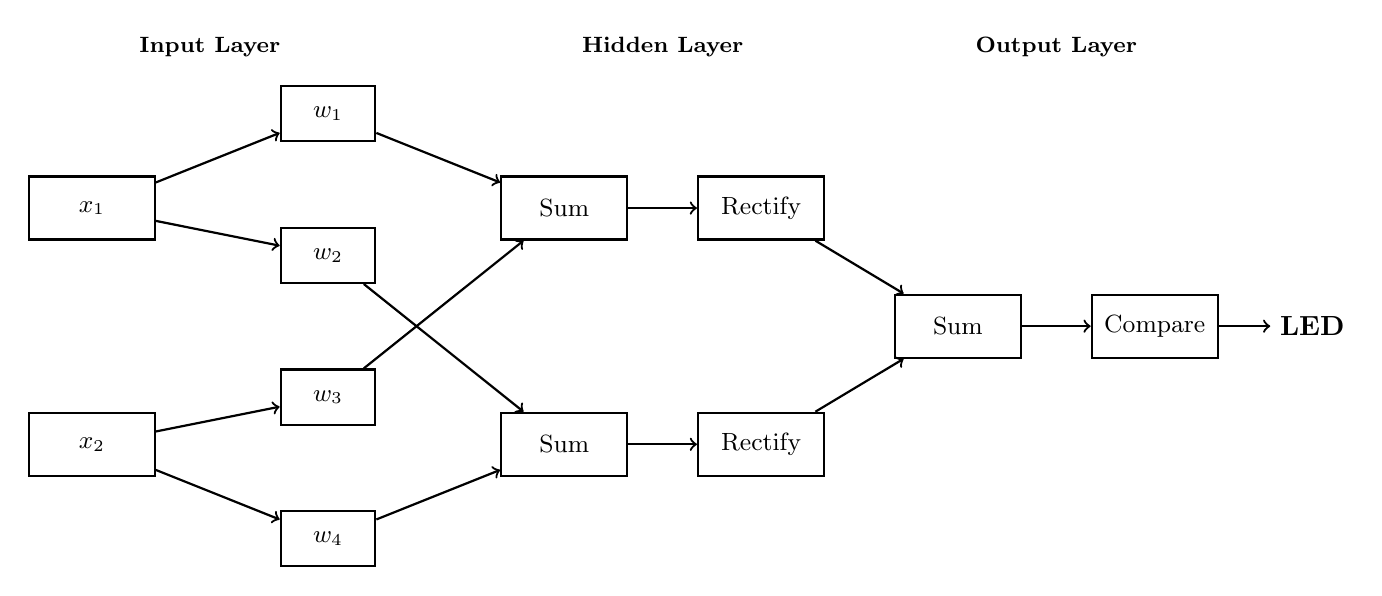
\begin{tikzpicture}[
    block/.style={draw, thick, minimum width=1.6cm, minimum height=0.8cm, align=center, font=\small},
    smallblock/.style={draw, thick, minimum width=1.2cm, minimum height=0.7cm, align=center, font=\small},
    arr/.style={->, thick},
]
% --- Column 1: Inputs ---
\node[block] (x1) at (0, 1.5) {$x_1$};
\node[block] (x2) at (0, -1.5) {$x_2$};

% --- Column 2: Weight Pots (4 boxes) ---
\node[smallblock] (w1) at (3, 2.7) {$w_1$};
\node[smallblock] (w2) at (3, 0.9) {$w_2$};
\node[smallblock] (w3) at (3, -0.9) {$w_3$};
\node[smallblock] (w4) at (3, -2.7) {$w_4$};

% --- Column 3: Summers ---
\node[block] (sum1) at (6, 1.5) {Sum};
\node[block] (sum2) at (6, -1.5) {Sum};

% --- Column 4: Rectifiers ---
\node[block] (act1) at (8.5, 1.5) {Rectify};
\node[block] (act2) at (8.5, -1.5) {Rectify};

% --- Column 5: Output Summer ---
\node[block] (sumout) at (11, 0) {Sum};

% --- Column 6: Comparator ---
\node[block] (comp) at (13.5, 0) {Compare};

% --- Column 7: LED ---
\node (led) at (15.5, 0) {\textbf{LED}};

% === Arrows: Inputs to Weight Pots (diagonal) ===
\draw[arr] (x1) -- (w1);
\draw[arr] (x1) -- (w2);
\draw[arr] (x2) -- (w3);
\draw[arr] (x2) -- (w4);

% === Arrows: Weight Pots to Summers (diagonal, crossing) ===
\draw[arr] (w1) -- (sum1);
\draw[arr] (w3) -- (sum1);
\draw[arr] (w2) -- (sum2);
\draw[arr] (w4) -- (sum2);

% === Arrows: Summers to Rectifiers (straight) ===
\draw[arr] (sum1) -- (act1);
\draw[arr] (sum2) -- (act2);

% === Arrows: Rectifiers to Output Summer (diagonal) ===
\draw[arr] (act1) -- (sumout);
\draw[arr] (act2) -- (sumout);

% === Arrows: Output Summer to Comparator to LED (straight) ===
\draw[arr] (sumout) -- (comp);
\draw[arr] (comp) -- (led);

% === Layer Labels ===
\node[font=\footnotesize\bfseries, above] at (1.5, 3.3) {Input Layer};
\node[font=\footnotesize\bfseries, above] at (7.25, 3.3) {Hidden Layer};
\node[font=\footnotesize\bfseries, above] at (12.25, 3.3) {Output Layer};

\end{tikzpicture}
\end{center}

Here is what each block does:

\begin{itemize}
    \itemsep2pt
    \item \textbf{Inputs} ($x_1$, $x_2$): Toggle switches selecting $+9$V (``on'') or $-9$V (``off'').
    \item \textbf{Weight Pots}: Potentiometers that scale each input by a value between $-1$ and $+1$. Turning the knob changes the weight.
    \item \textbf{Summers}: Op-amp circuits that add the weighted inputs together.
    \item \textbf{Rectifiers}: Diode circuits that pass only positive voltages and force negative ones to zero. This cutoff is what allows the network to make different ``decisions'' for different inputs --- without it, the whole network would just be one big addition, which is far too simple.
    \item \textbf{Comparator + Threshold}: Compares the output sum against an adjustable threshold voltage. If the sum exceeds the threshold, the LED turns on (output = 1). Otherwise, the LED is off (output = 0).
\end{itemize}

Over the rest of this lab, you will build each of these blocks as an analog circuit and then wire them together into a working neural network.

\subsection*{Dual Power Supply Setup}

Op-amps are \emph{active devices} that require external power. In this lab, we use a \emph{dual-sided supply}, providing $+9$\si{\volt} to $+V_{CC}$ and $-9$\si{\volt} to $-V_{CC}$. You can make this with two $9$V batteries connected in series:

\begin{figure}[h]
	\centering
	\begin{circuitikz}[scale=1,transform shape,american]
  	\draw (0,0) to[battery,*-o,v_=9V] (-4,0) node[anchor=south]{-$V_{CC}$};
  	\draw (4,0) node[anchor=south]{+$V_{CC}$} to[battery,o-,v_=9V] (0,0);
  	\draw (0,0) node[sground]{};
	\end{circuitikz}
	\caption{Making a dual-sided supply with two $9$V batteries}
	\label{fig:dual-sided-supply}
\end{figure}

\infotext{\linewidth}{Note the polarity of the battery terminals (connected positive to negative)}

Designate one half of your breadboard to use the $\pm 9$V rails. \textbf{Please remove the connections connecting all of your supply rails together on this section of the board.} The blue rails will be the reference node (ground), one of the red rails will be $+9$V, and the other red rail will be $-9$V. Figure \ref{fig:dual-supply-bb} is a breadboard diagram showing how to connect your batteries.

\begin{figure}[h]
	\centering
    \hspace{.5em}\includegraphics[width=0.9\linewidth]{dual-supply-bb_2.png}
	\caption{Making a dual-sided supply on a breadboard}
	\label{fig:dual-supply-bb}
\end{figure}

\warning{\linewidth}{Before connecting devices to the supply rails, check voltages with multimeter!}

Connect the black probe (COM) to the blue GND rail and you should measure +9V on one red rail and $-$9V on the other red rail. Make sure that you keep track of which is which. If you reverse the supply voltages going to the op amp chip, it can get very hot. \textbf{If the op-amp chip feels warm to the touch, disconnect the batteries immediately.}


\begin{questions}
    \begingradingrange{credit}
    \titledquestion{Comparator Light Switch}

The comparator is the simplest op-amp circuit: it compares two voltages and drives its output high or low. In our neural network, the comparator will form the \textbf{output decision} --- it compares the network's output sum against a threshold to decide whether the LED turns on.

Build the following circuit on your breadboard, which uses a light-dependent resistor (LDR) to control an LED:

\begin{figure}[h]
	\centering
	\begin{circuitikz}[scale=1.4, transform shape]
  	\draw (0, 0) node[op amp] (opamp) {\tiny TL072};
	\draw (opamp.+) to[short,-o] ++(-.5,0) node[anchor=east] {$v_+$};
 	\draw (opamp.out)  to[R,l=1k$\Omega$,/tikz/circuitikz/bipoles/length=1cm] ++(2.5,0) to[led] ++(0,-1.75) node[sground] {};
 	\draw (opamp.-) -- ++(-2,0) to[R,l=$R_X\hspace{.4cm}$,/tikz/circuitikz/bipoles/length=1cm] ++(0,2) node[opampuplbl] {$+9$V};
 node[sground] {};
 \draw (opamp.-) -- ++(-2,0) to[R,l_=$4.7$k$\Omega$,/tikz/circuitikz/bipoles/length=1cm] ++(0,-2) node[sground]{};
 	\draw (opamp.up) to[short] ++(0,0.5) node[opampuplbl] {$+9$V};
 	\draw (opamp.down) to[short] ++(0,-0.5) node[opampdownlbl] {$-9$V};
 	\draw (opamp.-) ++(-.7,0) node[anchor=south]{$v_-$};
 	\draw (opamp.-) ++(-2,1) circle (16pt);
	\end{circuitikz}
	\caption{Comparator Circuit with LED indicator at output and light-dependent voltage divider at the inverting input.}
	\label{fig:dccomp}
\end{figure}

This circuit uses the op amp in an open-loop configuration (i.e.\ no feedback). When the voltage at $v_+$ exceeds the voltage at $v_-$, the output will be driven to +9V and the LED will turn on. Otherwise, the LED will be off.

A voltage divider consisting of an LDR $R_X$ and a 4.7 k$\Omega$ resistor provides a voltage to the $v_-$ input. You will build a second voltage divider to provide $\approx4.5$V to the $v_+$ input. The comparator will compare $v_-$ to $v_+$ and then drive its output to either high (LED on) or low (LED off).

\begin{parts}
    \part[2] Measure $v_-$ using a digital multimeter, both when the LDR is well-lit and when the LDR is in the dark. What are the dark ($V_{dark}$) and light ($V_{light}$) voltages that you measured at $v_-$?
\medbreak
\textbf{$V_{dark}$} = \framebox[4cm][r]{\rule{0pt}{1cm}\si{\volt}} \quad \textbf{$V_{light}$} = \framebox[4cm][r]{\rule{0pt}{1cm}\si{\volt}}

    \part[10] Complete your light-switch circuit on your breadboard by adding a voltage divider to provide 4.5V to the $v_+$ input. The LED should have a different state when the LDR is well-lit versus when the LDR is in the dark.

    \medbreak
    \infotext{\linewidth}{You do not need to save this circuit. These components can be reused later.}

\end{parts}

\pagebreak

    \titledquestion{Buffer (Unity-Gain Amplifier)}

Before we build amplifiers, let's see why op-amps are useful even when the output voltage equals the input. The \emph{buffer} (also called a voltage follower) has very high input impedance and very low output impedance, which prevents one stage from ``loading'' another.

Construct the following circuit in Figure \ref{fig:vdiv}. The goal of this circuit is to divide down the initial voltage, $5$V, twice. Connect 5V from the breadboard power supply as the power supply for this circuit and measure $V_{A}$ and $V_{out}$ with your multimeter. $R_{1,2,3,4} = 10 \si{\kilo\ohm}$.

\begin{figure}[h]
	\centering
	\begin{circuitikz}[american,scale=1.25,transform shape]
		\draw (0,0) node[sground] {} to[vsource,invert,l=$5$V] ++(0,2) to[short] ++(1,0) to[R,l=$R_1$] ++(3,0) to[short, *-] ++(0,0) coordinate(center) to[R,l=$R_3$] ++(3,0) to[short, *-] ++(0,0) to[R,l=$R_4$] ++(0,-2) node[sground] {};
		\draw (center) node[anchor=south]{$V_{A}$} to[R,l_=$R_2$] ++(0,-2) node[sground] {};
		\draw (7.5,2.5) node[anchor=north] {$V_{out}$};
		\draw[blue, dashed] (8,-1.5) rectangle (4.5,3);
		\node[blue, above] at (6.25,-1.5){\footnotesize Voltage Divider};
		\draw[blue, dashed] (1,-1.5) rectangle (4.5,3);
		\node[blue, above] at (2.75,-1.5){\footnotesize Voltage Divider};
	\end{circuitikz}
	\caption{Cascading Voltage Dividers}
	\label{fig:vdiv}
\end{figure}

\begin{parts}
	\part[3] Measure the voltages $V_A$ and $V_{out}$ with your voltmeter:
	\medbreak
	\begin{center}
		\setlength{\tabcolsep}{14pt}
		\begin{tabular}{|c|c|} \hline
			\bm{$V_{A}$} & \bm{$V_{out}$} \\ \hline
		  \hspace{1cm} \rule{0pt}{3em} &  \hspace{1cm} \\ \hline
		\end{tabular}
	\end{center}

	\part[2] Is the circuit dividing the voltage in half twice (i.e.\ is $V_{out} = \frac{V_{in}}{4}$)? Explain why or why not.

	\makeemptybox{4cm}

\pagebreak

	\uplevel{Now we introduce a unity-gain buffer between the two voltage dividers. Build the circuit in Figure \ref{fig:buff2} and perform the same measurements. When you see an op amp from now on, the $+9$V and $-9$V supply rails are implied. $R_{1,2,3,4} = 1\si{\kilo\ohm}$.}

	\begin{figure}[h]
		\centering
		\begin{circuitikz}[american]
		\draw (5.19,2.5) node[op amp] (opamp) {\tiny \texttt{TL072}};
		\draw (0,0) node[sground] {} to[vsource,invert,l=$5$V] ++(0,2) to[short] ++(0.5,0) to[R,l=$R_1$] ++(3,0) to[short, *-] ++(0,0) node[] (center) {} to[short] (opamp.+);
		\draw (opamp.-) to[short,-] ++(0,1) coordinate (leftR)
  			  to[short] (leftR -| opamp.out)
 			  to[short,-*] (opamp.out) to[short,-] ++(0.5,0) -| ++(0,-0.49) to[short] ++(0,0) to[R,l=$R_3$] ++(3,0) node[anchor=south] {$V_{out}$} to[short, *-] ++(0,-0.5) to[R,l_=$R_4$] ++(0,-1.51) node[sground] {};
 		\draw (opamp.+) ++(-0.5,0) node[anchor=south]{$V_A$} to[short, -] ++(0,-0.5) to[R,l_=$R_2$] ++(0,-1.51) node[sground] {};
 		\draw[blue, dashed] (.65,-1.5) rectangle (3.85,5);
		\node[blue, above] at (2.25,-1.5){\footnotesize Voltage Divider};
		\draw[blue, dashed] (3.85,-1.5) rectangle (7,5);
		\node[blue, above] at (5.5,-1.5){\footnotesize Buffer};
		\draw[blue, dashed] (7,-1.5) rectangle (10.5,5);
		\node[blue, above] at (8.75,-1.5){\footnotesize Voltage Divider};
		\end{circuitikz}
		\caption{Consecutive voltage dividers separated by op amp buffer}
		\label{fig:buff2}
	\end{figure}

	\vspace{-\baselineskip}

    \part[3] Measure the voltages $V_A$ and $V_{out}$ with your voltmeter:
	\medbreak
	\begin{center}
		\setlength{\tabcolsep}{14pt}
		\begin{tabular}{|c|c|} \hline
			\bm{$V_{A}$} & \bm{$V_{out}$} \\ \hline
		  \hspace{1cm} \rule{0pt}{3em} & \hspace{1cm} \\ \hline
		\end{tabular}
	\end{center}

	\part[2] Explain why buffering the voltage dividers causes the correct level of voltage division. Refer to the input and output resistances of the op amp in your answer.

	\makeemptybox{4cm}
\end{parts}
\pagebreak

    \titledquestion{Amplifiers --- Non-Inverting and Inverting}

Now we introduce \emph{gain}. The non-inverting and inverting amplifier topologies use negative feedback and a resistor ratio to amplify a signal. Both are essential building blocks: the \textbf{inverting amplifier} in particular will serve as the \textbf{input inverter} in our neural network.

\subsection*{4A: Non-Inverting Amplifier}

The non-inverting amplifier amplifies without flipping the sign of the input. Assemble the circuit in Figure \ref{fig:non-inverting-amp} on your breadboard. Use a 1kHz 1$V_{pp}$ sine wave for $V_{in}$. Supply $\pm$9V to the op amp rails. Use a 20\si{\kilo\ohm} potentiometer for $R_f$ and a 1\si{\kilo\ohm} resistor for $R_i$.

\begin{figure}[h]
	\centering
	\begin{circuitikz}[scale=1.15,transform shape,american]
  		\draw (0, 0) node[op amp] (opamp) {\tiny TL072}
  			(opamp.-) to[R, l_=$R_i$] (-3, 0.5) node[sground] {};
  		\draw (opamp.-) to[short,*-] ++(0,1) coordinate (leftR)
  			to[vR, l=$R_f$, invert, mirror] (leftR -| opamp.out)
 			to[short,-*] (opamp.out) to[short,-o] ++(1,0) node[anchor=west] {$V_{out}$};
 		\draw (opamp.+) to[short, -] ++(-0.5,0) to[sV,l_=$V_{in}$ (\texttt{W1})] ++(0,-1.5) node[sground] {};
	\end{circuitikz}
	\caption{Non-Inverting Amplifier with Variable Gain}
	\label{fig:non-inverting-amp}
\end{figure}

\subsection{Using the Signal Generator and Oscilloscope}

In WaveForms, open the \texttt{Wavegen}. Read the following guide on how to configure and use the Signal Generator: \url{https://digilent.com/reference/test-and-measurement/guides/waveforms-waveform-generator}. Configure \texttt{Channel 1 (W1)} as follows:
\medbreak

\begin{center}
\begingroup
\setlength{\tabcolsep}{18pt}
\begin{tabular}{|l|l|}\hline
    \multicolumn{2}{|c|}{\texttt{Wavegen}} \\ \hline
    \multicolumn{2}{|c|}{Type: Sine} \\ \hline
    Frequency: 1kHz & Offset: 0V \\
    Amplitude: 1V & Phase: 0 deg \\ \hline
\end{tabular}
\endgroup
\end{center}

\medbreak
Connect \texttt{W1} to the positive terminal of $V_{in}$ and the AD3's \texttt{GND} to the negative terminal. Read the oscilloscope guide: \url{https://digilent.com/reference/test-and-measurement/guides/waveforms-oscilloscope}. Configure the following scope settings:
\medbreak
\begin{center}
\begingroup
\setlength{\tabcolsep}{18pt}
\begin{tabular}{|l|l|l|}\hline
\multicolumn{3}{|c|}{\texttt{Scope}} \\ \hline
    \textbf{Time} & \textbf{Channels} & \textbf{Channel Settings} \\ \hline
    Position: 0ms & Range: 500mV/div & Probe: 1X \\
    Base: 1ms/div & Offset: 0V & \\ \hline
\end{tabular}
\endgroup
\end{center}
\medbreak
Connect CH1 to $V_{in}$ and CH2 to $V_{out}$. Hit the \raisebox{-0.6ex}{\includegraphics[width=2cm]{waveforms_lab5_run.png}} button to start measuring.

\begin{parts}
\part[3] Set $R_f$ to $5\si{\kilo\ohm}$. Paste a screenshot of your oscilloscope plot. Make sure both CH1 and CH2 are enabled and have the same voltage range (volts/div), and that both waveforms are clearly visible.

\makessbox{5cm}

\part[2] Measure the peak-to-peak voltage at both the input and the output. What is the gain of this circuit?
\medbreak

\begin{tikzpicture}
	\draw[black] (0,0) rectangle (3,1.5);
	\draw[black] (0,2) rectangle (3,3.5);
	\draw[black] (-1.5,1.75) -- (3.25,1.75);
	\node[anchor=east] at (-0.15,2.75) {$V_{out}=$};
	\node[anchor=east] at (-0.15,0.75) {$V_{in}=$};
	\node[] at (-2.5,1.79) {\textbf{Gain =}};
	\node[] at (3.65,1.74) {\textbf{=}};
	\draw[black] (4.1,1) rectangle (7.1,2.5);
	\node[] at (2.7,0.3) {$V$};
	\node[] at (2.7,2.3) {$V$};
\end{tikzpicture}

\end{parts}

\pagebreak

\subsection*{4B: Inverting Amplifier --- The ANN Input Inverter}

The inverting amplifier flips the sign of the input. In our neural network, we need inverted copies of each input so that our weight pots can sweep from $-1$ to $+1$. If we only had the raw input, the pots could only give us weights from 0 to 1.

Assemble the circuit in Figure \ref{fig:ia} on your breadboard. Use a 10\si{\kilo\ohm} resistor for both $R_f$ and $R_i$. \textbf{Build 2 of these} --- these are the input inverters for the ANN. Only complete the following exercises for one of them.

\begin{figure}[h]
	\centering
	\begin{circuitikz}[scale=1.2,transform shape,american]
  	\draw (0, 0) node[op amp] (opamp) {\tiny TL072}
  		(opamp.-) to[R, l_=$R_i$] (-3, 0.5) to[sV,v_=$V_{in}$ (\texttt{W1})] ++(0,-1.5) node[sground] {};
  	\draw (opamp.-) to[short,*-] ++(0,1) coordinate (leftR)
  		to[R, l=$R_f$] (leftR -| opamp.out)
 		to[short,-*] (opamp.out) to[short,-o] ++(1,0) node[anchor=west] {$V_{out}$};
 	\draw (opamp.+) to[short, -] ++(-0.5,0) node[sground] {};
	\end{circuitikz}
	\caption{Inverting Amplifier with Fixed Gain}
	\label{fig:ia}
\end{figure}
\vspace{-\baselineskip}

Connect CH1 to the input and CH2 to the output.

\begin{parts}
\setcounter{partno}{2}

\part[3] Paste a screenshot of your oscilloscope plot. Make sure both CH1 and CH2 are enabled and have the same voltage range (volts/div), and that both waveforms are clearly visible.

\makessbox{5cm}
\medbreak

\part[3] Using the oscilloscope, measure the peak-to-peak voltage at both the input and the output. What is the gain of this circuit?
\medbreak

\begin{tikzpicture}
	\draw[black] (0,0) rectangle (3,1.5);
	\draw[black] (0,2) rectangle (3,3.5);
	\draw[black] (-1.5,1.75) -- (3.25,1.75);
	\node[anchor=east] at (-0.15,2.75) {$V_{out}=$};
	\node[anchor=east] at (-0.15,0.75) {$V_{in}=$};
	\node[] at (-2.5,1.79) {\textbf{Gain =}};
	\node[] at (3.65,1.74) {\textbf{=}};
	\draw[black] (4.1,1) rectangle (7.1,2.5);
	\node[] at (2.7,0.3) {$V$};
	\node[] at (2.7,2.3) {$V$};
\end{tikzpicture}

\part[3] Calculate the gain for the circuit in Figure \ref{fig:ia} given an ideal op-amp. Show that, for the resistance values used, the ideal gain matches the gain you measured.

\makeemptybox{2.5cm}

\end{parts}

\pagebreak

    \titledquestion{Inverting Summing Amplifier}

In our neural network, each hidden neuron needs to combine multiple weighted inputs into a single sum. The inverting summing amplifier does exactly this: it adds together several input voltages (each scaled by $-R_f / R_i$) and outputs their weighted sum.

Assemble the following circuit in Figure \ref{fig:sia} on your breadboard. Use a 4.7\si{\kilo\ohm} resistor for $R_f$ and 10\si{\kilo\ohm} for each $R_i$. This gives a gain of $-4.7/10 = -0.47$ per input. Use a 1kHz 1$V_{pp}$ sine wave for $V_{in}$ and a DC voltage of 5V for the second input.

\textbf{Build 3 of these} --- 2 for the hidden layer and 1 for the output layer of the ANN. Only take measurements on one.

\begin{figure}[h]
    \centering
    \begin{circuitikz}[scale=1.2,transform shape,american]
    % The Op-Amp
    \draw (0, 0) node[op amp] (opamp) {\tiny TL072};

    % Extending the inverting input line to create more room for the junction
    \draw (opamp.-) -- ++(-1, 0) coordinate (summing_node);

    % Input 1: Vin (W1)
    \draw (summing_node) -- ++(0, 1.5)
          to[R, l=$R_i$, *-] ++(-2, 0)
          to[sV, v_=$V_{in}$ (\texttt{W1})] ++(0,-1.5) node[sground] {};

    % Input 2: 5V DC Input
    \draw (summing_node) -- ++(0, -1.5)
          to[R, l=$R_i$, *-] ++(-2, 0)
          to[V, v_=5V] ++(0,-1.5) node[sground] {};

    % Feedback Loop
    \draw (opamp.-) to[short,*-] ++(0,1.8) coordinate (leftR)
        to[R, l=$R_f$] (leftR -| opamp.out)
        to[short,-*] (opamp.out) to[short,-o] ++(1,0) node[anchor=west] {$V_{out}$};

    % Grounding the Non-Inverting Input
    \draw (opamp.+) to[short, -] ++(-0.5,0) node[sground] {};

    \end{circuitikz}
    \caption{Inverting Summing Amplifier}
    \label{fig:sia}
\end{figure}

Connect CH1 to $V_{in}$ and CH2 to $V_{out}$.

\begin{parts}
\part[3] Paste a screenshot of your oscilloscope plot. Make sure both CH1 and CH2 are enabled and have the same voltage range (volts/div), and that both waveforms are clearly visible.

\makessbox{5cm}

\end{parts}

\pagebreak

    \titledquestion{Diode Rectifier}

Our neural network needs a way to introduce a \emph{cutoff} so that it can make different ``decisions'' depending on the input. Without this, the entire network would reduce to one big weighted sum, which is far too simple to represent interesting functions. To add this cutoff, we will use a \textbf{diode rectifier}: a circuit that passes positive voltages through but forces all negative voltages to zero.

This is actually very close to a function used in real artificial neural networks (including large language models like ChatGPT), called a \textbf{ReLU} (Rectified Linear Unit):

\begin{center}
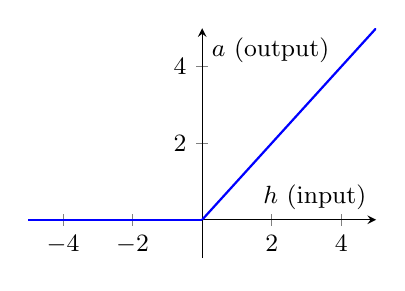
\begin{tikzpicture}
    \begin{axis}[
        width=6cm, height=4.5cm,
        xlabel={$h$ (input)}, ylabel={$a$ (output)},
        axis lines=center,
        xmin=-5, xmax=5, ymin=-1, ymax=5,
        xtick={-4,-2,0,2,4}, ytick={0,2,4},
        every axis plot/.append style={thick},
        font=\small,
    ]
    \addplot[blue, domain=-5:0] {0};
    \addplot[blue, domain=0:5] {x};
    \end{axis}
\end{tikzpicture}

$a = \max(0,\; h)$
\end{center}

Our diode version isn't perfect --- it has a $\sim$0.6V dead zone due to the diode's forward voltage drop --- but this isn't critical; the network can still represent any function.

Assemble the circuit in Figure \ref{fig:rectifier} on your breadboard. Use a 1N4148 signal diode and a 10\si{\kilo\ohm} pull-down resistor. \textbf{Build 2 of these} --- one per hidden neuron.

For testing, connect a 1kHz 5$V_{pp}$ sine wave from the signal generator to the input.

\begin{figure}[h]
    \centering
    \begin{circuitikz}[scale=1.3, transform shape, american]
        % Input
        \draw (-3, 0) to[sV, v_=$V_{in}$ (\texttt{W1})] ++(0,-2) node[sground] {};
        \draw (-3, 0) to[short, -o] ++(-0.5, 0) node[left] {In};
        \draw (-3, 0) to[diode, l=1N4148] ++(3, 0) coordinate (out_node);

        % Output
        \draw (out_node) to[short, -o] ++(1, 0) node[right] {Out ($a$)};

        % Pull-down resistor
        \draw (out_node) to[R, l_=10k$\Omega$, *-] ++(0, -2) node[sground] {};
    \end{circuitikz}
    \caption{Bare diode rectifier with pull-down resistor. When $V_{in} > 0.6$V, the diode conducts and the output follows the input (minus the diode drop). When $V_{in} < 0.6$V, the diode is reverse-biased and the pull-down resistor holds the output at 0V.}
    \label{fig:rectifier}
\end{figure}

Connect CH1 to the input and CH2 to the output.

In WaveForms, set the Wavegen to Sine with $f = 1$kHz and amplitude = 5V. For the scope, set your CH1 range to 1V/div.

\pagebreak
\begin{parts}
\part[3] Paste a screenshot of your oscilloscope showing the rectification of the sine wave. Both the input and output waveforms should be clearly visible.

\makessbox{5cm}
\medbreak

\part[2] Explain what the circuit does: what happens to positive input voltages? What happens to negative input voltages? How does the diode accomplish this?

\makeemptybox{3cm}
\end{parts}

\pagebreak

    % q6_ann.tex

% --- Custom Pic Definitions ---
\tikzset{
    invamp/.pic={
        \draw [thick, fill=white] (-1,-1) rectangle (1,1);
        \node [font=\small\bfseries, align=center] at (0,0) {Inv\\Amp};
        \coordinate (-in) at (-1, 0);
        \coordinate (-out) at (1, 0);
        \node [right, font=\tiny] at (-in) {In};
        \node [left, font=\tiny] at (-out) {Out};
    },
    sumamp/.pic={
        \draw [thick, fill=white] (-1,-1.2) rectangle (1,1.2);
        \node [font=\small\bfseries, align=center] at (0,0) {Sum\\Amp};
        \coordinate (-in1) at (-1, 0.5);
        \coordinate (-in2) at (-1, -0.5);
        \coordinate (-out) at (1, 0);
        \node [right, font=\tiny] at (-in1) {In1};
        \node [right, font=\tiny] at (-in2) {In2};
        \node [left, font=\tiny] at (-out) {Out};
    },
    dioderect/.pic={
        \draw [thick, fill=white] (-1,-1) rectangle (1,1);
        \node [font=\small\bfseries, align=center] at (0,0) {Diode\\Rect};
        \coordinate (-in) at (-1, 0);
        \coordinate (-out) at (1, 0);
        \node [right, font=\tiny] at (-in) {In};
        \node [left, font=\tiny] at (-out) {Out};
    }
}

\titledquestion{Putting It All Together --- The Analog Neural Network}

Now we connect all of our building blocks into the full neural network described in the Introduction. To keep the schematics readable, we will use the following block abstractions for circuits you have already built:

\subsection*{Circuit Abstractions}

% --- EQUIVALENCY 1: INVERTING AMPLIFIER ---
\begin{figure}[h!]
    \centering
    \begin{minipage}{0.55\textwidth}
        \centering
        \begin{circuitikz}[scale=0.8, transform shape, american]
            \draw (0,0) node[op amp] (opamp) {\tiny{TL072}};
            \draw (opamp.-) to[R, l=$R_i$, *-o] ++(-2, 0) node[left] {$V_{in}$};
            \draw (opamp.+) to[short] ++(-0.5,0) node[sground] {};
            % Feedback Loop
            \draw (opamp.-) -- ++(0, 1.5) coordinate (top)
                  to[R, l=$R_f$] (top -| opamp.out)
                  -- (opamp.out)
                  to[short, -o] ++(0.5, 0) node[right] {Out};
        \end{circuitikz}
    \end{minipage}
    \begin{minipage}{0.1\textwidth}
        \centering \Huge $\Longrightarrow$
    \end{minipage}
    \begin{minipage}{0.25\textwidth}
        \centering
        \begin{circuitikz}
            \draw (0,0) pic {invamp};
        \end{circuitikz}
    \end{minipage}
    \caption{Abstraction of the Inverting Amplifier ($R_i = R_f = 10$k$\Omega$, gain $= -1$)}
\end{figure}

% --- EQUIVALENCY 2: SUMMING AMPLIFIER ---
\begin{figure}[h!]
    \centering
    \begin{minipage}{0.55\textwidth}
        \centering
        \begin{circuitikz}[scale=0.8, transform shape, american]
            \draw (0, 0) node[op amp] (opamp) {\tiny TL072};
            % Move summing node slightly left of the op-amp input
            \draw (opamp.-) -- ++(-0.5, 0) coordinate (summing_node);

            % Input 1
            \draw (summing_node) -- ++(0, 1) -- ++(-0.5,0)
                  to[R, l=$R_i$, -o] ++(-1.5, 0) node[left] {$V_{in1}$};

            % Input 2
            \draw (summing_node) -- ++(0, -1) -- ++(-0.5,0)
                  to[R, l=$R_i$, -o] ++(-1.5, 0) node[left] {$V_{in2}$};

            % Feedback
            \draw (opamp.-) to[short,*-] ++(0,1.5) coordinate (leftR)
                to[R, l=$R_f$] (leftR -| opamp.out)
                to[short,-*] (opamp.out) to[short,-o] ++(0.5,0) node[right] {$V_{out}$};
            \draw (opamp.+) to[short, -] ++(-0.2,0) node[sground] {};
        \end{circuitikz}
    \end{minipage}
    \begin{minipage}{0.1\textwidth}
        \centering \Huge $\Longrightarrow$
    \end{minipage}
    \begin{minipage}{0.25\textwidth}
        \centering
        \begin{circuitikz}
            \draw (0,0) pic {sumamp};
        \end{circuitikz}
    \end{minipage}
    \caption{Abstraction of the Inverting Summing Amplifier ($R_i = 10$k$\Omega$, $R_f = 4.7$k$\Omega$, gain $= -0.47$ per input)}
\end{figure}

% --- EQUIVALENCY 3: DIODE RECTIFIER ---
\begin{figure}[h!]
    \centering
    \begin{minipage}{0.55\textwidth}
        \centering
        \begin{circuitikz}[scale=0.8, transform shape, american]
            % Input
            \draw (-2, 0) node[left] {In} to[short, o-] ++(0.5,0)
                to[diode, l=1N4148] ++(2.5, 0) coordinate (out_node);
            % Output
            \draw (out_node) to[short, -o] ++(1, 0) node[right] {Out};
            % Pull-down
            \draw (out_node) to[R, l_=10k$\Omega$, *-] ++(0, -2) node[sground] {};
        \end{circuitikz}
    \end{minipage}
    \begin{minipage}{0.1\textwidth}
        \centering \Huge $\Longrightarrow$
    \end{minipage}
    \begin{minipage}{0.25\textwidth}
        \centering
        \begin{circuitikz}
            \draw (0,0) pic {dioderect};
        \end{circuitikz}
    \end{minipage}
    \caption{Abstraction of the Diode Rectifier (1N4148 + 10k$\Omega$ pull-down)}
\end{figure}

\newpage
\subsection*{7A: Input Stage}

Each input switch selects $+9$V or $-9$V. An inverting amplifier creates the negated copy of each input. Four potentiometers blend the raw and inverted inputs, allowing each weight to sweep from $-1$ to $+1$.

Wire up the circuit as shown below. Once complete, use a DMM to verify that each wiper ($w_1$ through $w_4$) can sweep from approximately $+9$V to $-9$V as you turn the pot.

\begin{center}
\resizebox{\linewidth}{!}{%
\begin{circuitikz}[american, transform shape, scale=0.8]

% ---- Layout Coordinates ----
\def\xSrc{-2.5}
\def\xInv{0}
\def\xRaw{-1.5}  % junction point, must be left of inv amp box (box left edge = \xInv - 1)
\def\xPot{4}

\def\yTop{2.2}
\def\yBot{-2.2}

% ==========================
% TOP CHANNEL (Input 1)
% ==========================

% 1. DRAW AMPLIFIER FIRST
\draw (\xInv,\yTop) pic (OA1) {invamp};

% 2. Input Source & Switch
\draw (\xSrc, \yTop) node[spdt, rotate=180] (SW1) {};
\draw (SW1.in) -- (\xRaw, \yTop) coordinate (raw1) -- (OA1-in);
\draw (SW1.out 2) -- ++(-0.5,0) node[left] {$+9$V};
\draw (SW1.out 1) -- ++(-0.5,0) node[left] {$-9$V};

% 3. Potentiometers (W1, W2)
\draw (\xPot, \yTop+1.8) to[pR, n=W1, l_=W1] (\xPot, \yTop+0.5);
\draw (\xPot, \yTop-0.5) to[pR, n=W2, l_=W2] (\xPot, \yTop-1.8);

% 4. WIRING
\draw (OA1-out) -- ++(1,0) coordinate (out_split1);
\draw (out_split1) |- ([yshift=-0.1cm]W1.east);
\draw (out_split1) |- ([yshift=-0.1cm]W2.east);

% Raw input to pot tops: up over inv amp box, then split right to each pot
\draw (raw1) |- ++(3, 1.5) coordinate (over1);
\draw (over1) |- ([yshift=0.1cm]W1.west);
\draw (over1) |- ([yshift=0.1cm]W2.west);
\node[circ] at (raw1) {};

% Label Wipers with Outputs
\draw (W1.wiper) -- ++(0.5,0) node[right, font=\small] {$\; \; w_1$} to[short, -o] ++(0.2,0);
\draw (W2.wiper) -- ++(0.5,0) node[right, font=\small] {$\; \;w_2$} to[short, -o] ++(0.2,0);

% ==========================
% BOTTOM CHANNEL (Input 2)
% ==========================

% 1. DRAW AMPLIFIER FIRST
\draw (\xInv,\yBot) pic (OA2) {invamp};

% 2. Input Source & Switch
\draw (\xSrc, \yBot) node[spdt, rotate=180] (SW2) {};
\draw (SW2.in) -- (\xRaw, \yBot) coordinate (raw2) -- (OA2-in);
\draw (SW2.out 2) -- ++(-0.5,0) node[left] {$+9$V};
\draw (SW2.out 1) -- ++(-0.5,0) node[left] {$-9$V};

% 3. Potentiometers (W3, W4)
\draw (\xPot, \yBot+1.8) to[pR, n=W3, l_=W3] (\xPot, \yBot+0.5);
\draw (\xPot, \yBot-0.5) to[pR, n=W4, l_=W4] (\xPot, \yBot-1.8);

% 4. WIRING
\draw (OA2-out) -- ++(1,0) coordinate (out_split2);
\draw (out_split2) |- ([yshift=-0.1cm]W3.east);
\draw (out_split2) |- ([yshift=-0.1cm]W4.east);

% Raw input to pot tops: up over inv amp box, then split right to each pot
\draw (raw2) |- ++(3, 1.5) coordinate (over2);
\draw (over2) |- ([yshift=0.1cm]W3.west);
\draw (over2) |- ([yshift=0.1cm]W4.west);
\node[circ] at (raw2) {};

% Label Wipers with Outputs
\draw (W3.wiper) -- ++(0.5,0) node[right, font=\small] {\; \;$w_3$} to[short, -o] ++(0.2,0);
\draw (W4.wiper) -- ++(0.5,0) node[right, font=\small] {\; \;$w_4$} to[short, -o] ++(0.2,0);

\end{circuitikz}
}
\end{center}

\newpage
\subsection*{7B: Hidden Layer}

Connect the weight pot outputs ($w_1$ through $w_4$) to the inverting summers. The summer outputs pass through diode rectifiers, which cut off all negative voltages.

\begin{center}
\resizebox{\linewidth}{!}{%
\begin{circuitikz}[american, transform shape, scale=0.8]

% ---- Layout Coordinates ----
\def\xSum{0}
\def\xRect{4}

\def\yTop{2}
\def\yBot{-2}

% ==========================
% TOP CHANNEL
% ==========================
% Summing Amp
\draw (\xSum, \yTop) pic (Sum1) {sumamp};
% Inputs
\draw (Sum1-in1) to[short, -o] ++(-0.5,0) node[left] {$w_1$};
\draw (Sum1-in2) to[short, -o] ++(-0.5,0) node[left] {$w_3$};

% Diode Rectifier
\draw (\xRect, \yTop) pic (Rect1) {dioderect};

% Connections
\draw (Sum1-out) -- (Rect1-in);
\draw (Rect1-out) to[short, -o] ++(0.5,0) node[right] {$a_1$};


% ==========================
% BOTTOM CHANNEL
% ==========================
% Summing Amp
\draw (\xSum, \yBot) pic (Sum2) {sumamp};
% Inputs
\draw (Sum2-in1) to[short, -o] ++(-0.5,0) node[left] {$w_2$};
\draw (Sum2-in2) to[short, -o] ++(-0.5,0) node[left] {$w_4$};

% Diode Rectifier
\draw (\xRect, \yBot) pic (Rect2) {dioderect};

% Connections
\draw (Sum2-out) -- (Rect2-in);
\draw (Rect2-out) to[short, -o] ++(0.5,0) node[right] {$a_2$};

\end{circuitikz}
}
\end{center}

\newpage
\subsection*{7C: Output Stage}

Connect the rectifier outputs ($a_1$, $a_2$) to the output inverting summer. Then connect the output summer to the non-inverting input of the comparator. Wire the threshold pot between $V+$ and $V-$ (wiper to the comparator's inverting input). Finally, connect the comparator output to the LED through a 4.7k$\Omega$ current-limiting resistor.

\begin{center}
\resizebox{\linewidth}{!}{%
\begin{circuitikz}[american, transform shape, scale=0.8]

% ---- Comparator ----
\draw (6,0) node[op amp] (OA6) {\tiny{TL072}};

% ---- Summing Amp (placed so output y exactly matches OA6.+) ----
\path let \p1=(OA6.+) in (0, \y1) pic (SumFinal) {sumamp};
% Inputs from previous stage
\draw (SumFinal-in1) to[short, -o] ++(-0.5,0) node[left] {$a_1$};
\draw (SumFinal-in2) to[short, -o] ++(-0.5,0) node[left] {$a_2$};

% Connect Summing Amp Output to Non-Inverting Input (+)
\draw (SumFinal-out) -- (OA6.+);

% ---- Threshold Pot ----
\draw (OA6.-) -- ++(0,1) coordinate (trim_connect);
\path (trim_connect)-- ++(-1.5,0) coordinate (pot_top);
\draw (pot_top) to[pR, n=Trim, l=T 10k, mirror] ++(0,2) node[vcc]{+9V};
\draw (Trim.west) -- ++(0,-0.5) node[vee]{-9V};
\draw (Trim.wiper) -- (trim_connect);

% ---- Output LED Circuit ----
\draw (OA6.out) to[R, l=4.7k] ++(2.5,0)
      to[led, l=Red LED, fill=red] ++(0,-2) node[vee]{-9V};

\end{circuitikz}
}
\end{center}

\newpage
\subsection*{7D: Check-off}

An online tuning tool is available at:
\begin{center}
\url{https://nathanmehaffy.github.io/neural-net-lab/}
\end{center}
This tool uses \textbf{gradient descent} --- the same optimization algorithm used to train real neural networks --- to find weight and threshold values that implement any target Boolean function. You will use it to program your circuit.

\savecircuit

\begin{parts}
\part[20] \textbf{Check-off}: Open the tuning tool and select \textbf{XOR} as the target function. Click \textbf{Optimize}, then use a DMM to transfer the resulting weight and threshold values to your physical circuit. Demonstrate to a TA that your circuit correctly implements XOR by cycling through all four input combinations. Repeat for \textbf{NAND}.
\end{parts}

\subsection*{7E: Training the Network by Hand (Bonus)}

The manual tuning procedure below approximates gradient descent --- so by following it, you are doing roughly the same process used to train a real neural network, but by hand:

\begin{enumerate}
    \item Set all weights to 0 (pot knobs to the middle).
    \item Find the spot where turning the threshold pot flips the output
    (should be near 0) and put it slightly past that so the output LED is on.
    \item Cycle through the four possible inputs until you find one for which
    the output is incorrect. (If none are incorrect, you are done!)
    \item Determine which of the two hidden neurons to update:
    if the input is (0, 0) or (0, 1), update the first hidden neuron.
    If the input is (1, 0) or (1, 1), update the second hidden neuron.
    \item Find the gradient: for each of the two weight pots connected to
    the hidden neuron you selected, look at the input connected to that weight.
    If the input is on, the gradient for that weight is positive. If the input
    is off, the gradient for that weight is negative.
    \item Turn each of the two pots about a quarter-turn in the direction of
    the gradient. The exact amount doesn't matter.
    \item Repeat from step 3 until your network represents the target function.
    If you end up with the inverse of your target function, your network is
    wired backwards. Don't worry --- just repeat the process but turn the weights
    in the opposite direction in step 6.
\end{enumerate}

\begin{parts}
\setcounter{partno}{1}
\bonuspart[5] \textbf{Bonus Check-off}: Train your ANN to perform both \textbf{XOR} and \textbf{NAND} by hand using the procedure above, in front of a TA.
\end{parts}

    \endgradingrange{credit}
\end{questions}

\end{document}
